% Chapter Template

\chapter{Methods} % Main chapter title

\label{Chapter2} % Change X to a consecutive number; for referencing this chapter elsewhere, use \ref{ChapterX}

%----------------------------------------------------------------------------------------
%	SECTION 1
%----------------------------------------------------------------------------------------

\section{Reynolds Number}

Our first goal is to find a set of points we will refer to as points of interests. To start this we need to calculate the Reynolds-Number (\ensuremath{RE}) \ref{eq:1} of each voxel in every time-step.
Where we take the product of  \ensuremath{p} as the density of the fluid, \ensuremath{u} is the flow speed of the fluid, and \ensuremath{L} as the characteristic linear dimension, and using $\mu$ as the divisor to get the \ensuremath{RE} for that voxel in that time-step. It should be noted that for constancy in our simulations \ensuremath{L} is calculated by calculating the average length of the sides of each voxel  (\ensuremath{\sqrt[3]{l*w*h}}) changing this value can effect he discrete values but it does not alter the distribution on values. 

\begin{equation}\label{eq:1}
RE  = \frac{puL} {\mu} 
\end{equation}

Now that we have Reynolds Number of each time-step \ensuremath{RE_t} where \ensuremath{t} is the index number referencing a time value.  We find the mean value for each voxel \ref{eq:2} then threshold the data in to two categories \ensuremath{RE>150} as turbulent flow and \ensuremath{0<RE<=40}  as laminar flow, we exclude \ensuremath{RE} values of zero because they indicative of an area that is within an obstruction (e.g. underground, inside of a building). Next we need to compile a list of the index positions for the thresholded data and convert each set of indexes to positions. \color{red} [Better way to state this?] \color{black} 
\begin{equation} \label{eq:2}
RE_{mean} = \frac{1}{n} \sum_{i=1}^{n} RE_{i}=\frac{1}{n}\left(RE_{1}+\cdots+RE_{n}\right)
\end{equation} 

 We are then able to run a Clustering algorithm on each category of positions, in this case we use k-means on. This groups all points in to \ensuremath{k} groups while minimizing the distance between a point and that groups centroid. We calculate the value of \ensuremath{k} by taking the \ensuremath{\frac{1}{2}\sqrt[3]{I*J*K}} where \ensuremath{I,J} and \ensuremath{K} are the number of voxels in the x, y and z axis respectively. We then are able to take the centriod from each cluster and and we will refer to these as our points of interest from now on.

\begin{figure}
\centering
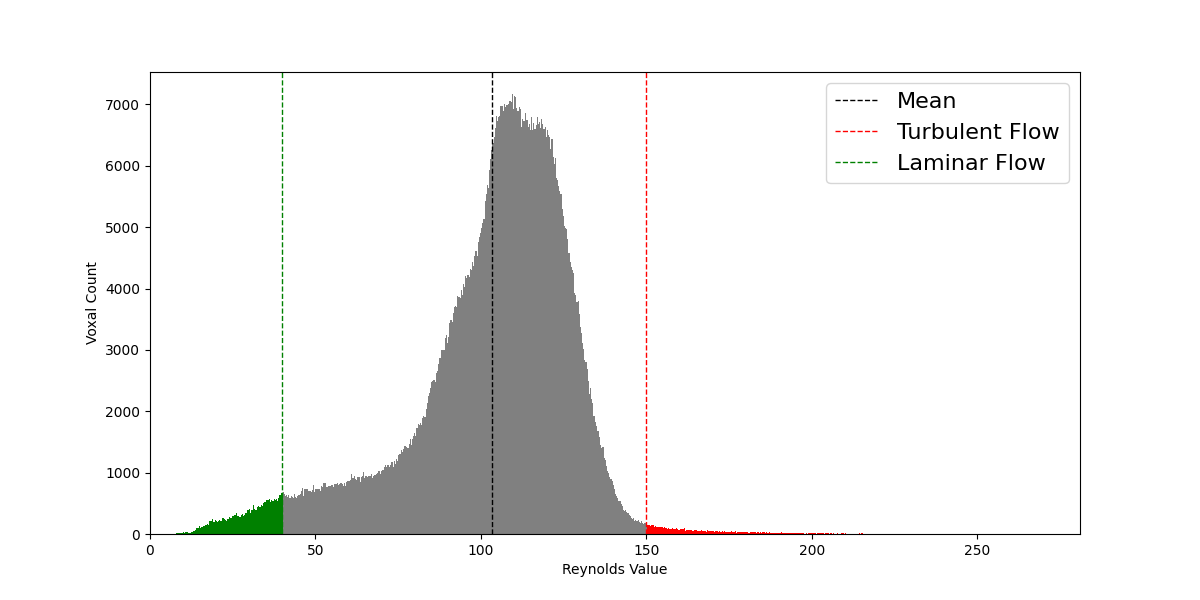
\includegraphics[scale=.25]{Figures/MethodsGraph.png}
\decoRule
\caption[A histogram]{Mean Reynolds Values Histgram}
\label{fig:MHistgram}
\end{figure}

\begin{figure}
\centering
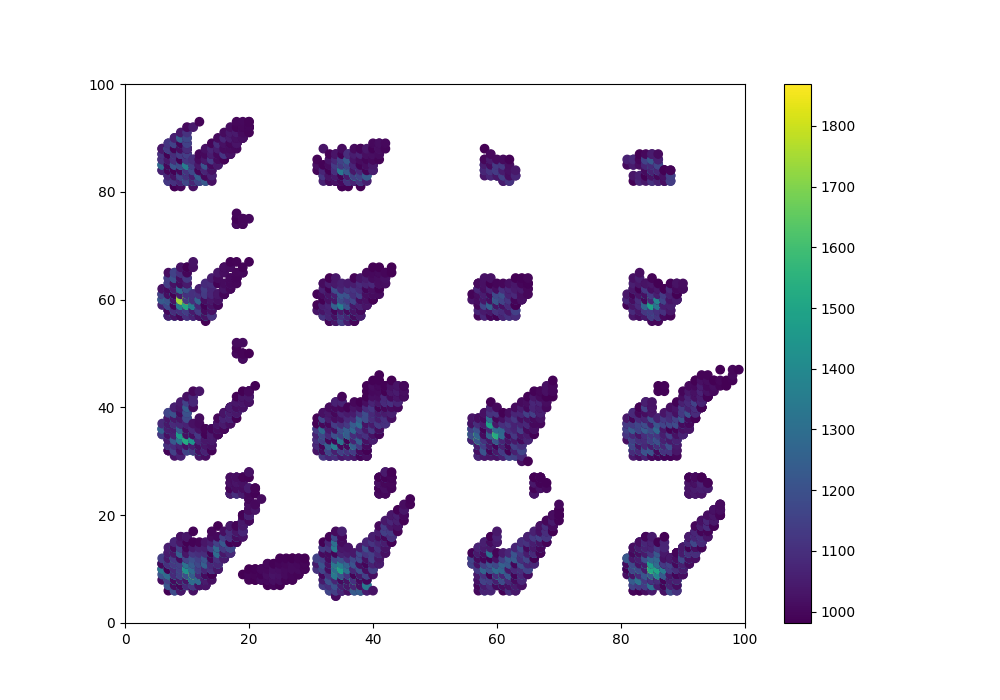
\includegraphics[scale=.25]{Figures/Turb2d.png}
\decoRule
\caption[Turbulent Air Flow Skatter Plot]{A plot showing areas of turbulent air flow}
\label{fig:MTurbulentflow}
\end{figure}
%-----------------------------------
%	SECTION 2
%-----------------------------------
\section{Pathline Calculations}


Now that we have calculated these points of interest we can use an Ordinary Differential Equations (ODE) to calculate the streamlines. We will use a fith-order Ruge-Kutta method for adaptive time steps and to minimize errors in calculations. We are able to use forward and reverse integration to calculate path lines for every time-step that pass though these points of interest. After intergrating in both directions we then combine the posting and time data for each pathline while also adding in the Reynolds Number for each point as well. We store all of this data in hdf5 files so it can be quickly loaded in to our visualization pipeline in Unity.

%-----------------------------------
%	SECTION 3
%-----------------------------------
\section{Unity Visualization}
Once we read in all of the data for each point in each pathline in to unity. We determine the largest (\ensuremath{RE_{max}}) and smallest (\ensuremath{RE_{min}}) value that within the data set, with the minimum and maximum values we are now able to calculate the a color value for each segment of the pathlines. To do so we have to calculate the interpolant value  within the range [\ensuremath{RE_{min}}, \ensuremath{RE_{max}}]\ref{eq:3}. This provides us with a value between [0,1] and then we can map this value to a color on a  perceptually uniform color map \color{red} [We use  vega's magma color map with 8 colors] \color{black} For each time step we load in the respective data for all \ensuremath{k} pathlines. to resolve the issue of being able to see orientation but not true directionality of a pathline (a line going left to right looks identical to a line going right to left) We segment each pathline in to n-1 line segments
(e.g. \ensuremath{P_0\rightarrow P_1},\ensuremath{P_1 \rightarrow P_2},...,\ensuremath{P_{n-2} \rightarrow P_{n-1}}) 
we then adjust the starting width of each line segment to be the average length of a voxel and the ending width zero, this give the lines a conical shape to indicate the directionality. We then build a color gradient and apply it to the  texture from point to point with the pre-calculated color map. This resolves the issues with un-clear directionality in other visualization methods as previously discussed. We are able to compile and build our Unity system in to an executable file that allows for the end user to run the file and  just type in the directory of the hdf5 files output discussed previously. Then they are able to move around and the environment in either Virtual Reality or just by using the mouse and keyboard.


\begin{equation} \label{eq:3}
f(RE_{min},RE_{max},RE_{value}) = \frac{RE_{value}-RE_{min}}{RE_{max}-RE_{min}}
\end{equation} 